\documentclass[tikz,border=2pt]{standalone}
\usepackage{amsmath,amssymb}
\usepackage{tikz}
\usetikzlibrary{arrows.meta}

\begin{document}
% Schwarz / Clairaut: when the mixed partials are continuous, differentiating first in x then
% in y gives the same result as the other order — the square commutes.
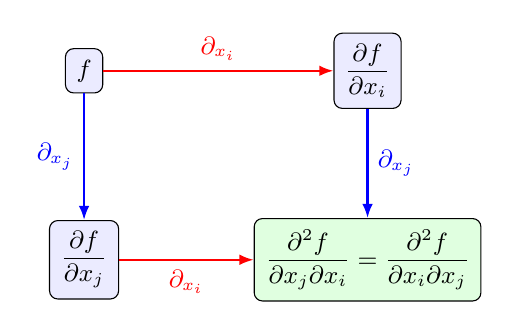
\begin{tikzpicture}[every node/.style={font=\small}, >={Latex[length=1.8mm]}, lvl/.style={draw, rounded corners=3pt, fill=blue!8, inner sep=4pt}]
	\node[lvl] (f) at (0,0) {$f$};
	\node[lvl] (fx) at (3.6,0) {$\dfrac{\partial f}{\partial x_i}$};
	\node[lvl] (fy) at (0,-2.4) {$\dfrac{\partial f}{\partial x_j}$};
	\node[lvl, fill=green!12] (fxy) at (3.6,-2.4) {$\dfrac{\partial^2f}{\partial x_j\partial x_i}=\dfrac{\partial^2f}{\partial x_i\partial x_j}$};
	\draw[->, thick, red] (f) -- (fx) node[midway, above] {$\partial_{x_i}$};
	\draw[->, thick, blue] (fx) -- (fxy) node[midway, right] {$\partial_{x_j}$};
	\draw[->, thick, blue] (f) -- (fy) node[midway, left] {$\partial_{x_j}$};
	\draw[->, thick, red] (fy) -- (fxy) node[midway, below] {$\partial_{x_i}$};
\end{tikzpicture}
\end{document}
